\documentclass[12pt]{article}
\usepackage{tikz}
\usepackage{amsmath}
% Underlining package
\usepackage{ulem}
\usetikzlibrary{calc}
\usepackage[a4paper, portrait, margin=1cm]{geometry}
\usepackage{fancyhdr}

\def \HeadingQuestions {\section*{\Large Name: \underline{\hspace{8cm}} \hfill Date: \underline{\hspace{3cm}}} \vspace{-3mm}
{Angles in a Triangle: Questions} \vspace{1pt}\hrule}

% raise footer with page number; no header
\fancypagestyle{myfancypagestyle}{
  \fancyhf{}% clear all header and footer fields
  \renewcommand{\headrulewidth}{0pt} % no rule under header
  \fancyfoot[C] {\thepage} \setlength{\footskip}{6pt} % raise page number 6pt
}
\pagestyle{myfancypagestyle}  % apply myfancypagestyle

\newcounter{minipagecount}

\begin{document}
\HeadingQuestions
\vspace{8mm}

\begin{minipage}{0.55\textwidth}
  \refstepcounter{minipagecount}
  \noindent{(\theminipagecount)}\quad
  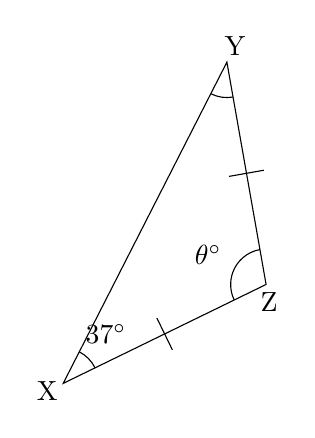
\begin{tikzpicture}[scale=1.5, baseline=(current bounding box.north)]
      \pgfmathsetmacro{\angleA}{37}
      \pgfmathsetmacro{\angleB}{37}
      \pgfmathsetmacro{\angleC}{106}
      \pgfmathsetmacro{\sideC}{3.052436047555899}
      \pgfmathsetmacro{\rotationAngle}{243}
  
    
      \begin{scope}[rotate=\rotationAngle]
        \coordinate (A) at (0,0);
        \coordinate (B) at (\sideC,0);
        \coordinate (C) at (intersection cs: first line={(A)--($(A)+(\angleA:4cm)$)}, second line={(B)--($(B)+(180-\angleB:4cm)$)});
        \draw (A) -- (B) -- (C) -- cycle;
        
        % Mark angles with arcs
        \draw ($(A)!0.3cm!(B)$) arc [start angle=0, end angle=\angleA, radius=0.3cm];
        \draw ($(B)!0.3cm!(C)$) arc [start angle=180-\angleB, end angle=180, radius=0.3cm];
        \draw ($(C)!0.3cm!(A)$) arc [start angle=180+\angleA, end angle=360-\angleB, radius=0.3cm];
        
        % Label angles
        \node at ($(A)!-0.15cm!(B)$) {Y};
        \node at ($(B)!-0.15cm!(C)$) {X};
        \node at ($(C)!-0.15cm!(A)$) {Z};
        
        % Mark angles in degrees
        \coordinate (midBC) at ($(B)!0.5!(C)$);
        \node at ($(A)!0.55cm!(midBC)$) {};
    
        \coordinate (midAC) at ($(A)!0.5!(C)$);
        \node at ($(B)!0.55cm!(midAC)$) {37$^\circ$};
    
        \coordinate (midAB) at ($(A)!0.5!(B)$);
        \node at ($(C)!0.55cm!(midAB)$) {$\theta ^\circ$};

        % Draw hash mark perpendicular to line AB at its midpoint
        \draw[black] ($(midAC)!1.5mm!90:(A)$)--($(midAC)!1.5mm!-90:(A)$);
              
        % Add hash marks on side AC
        \draw[black] ($(midBC)!1.5mm!90:(B)$)--($(midBC)!1.5mm!-90:(B)$);
              
      \end{scope}
    \end{tikzpicture}
\end{minipage}%
\hfill
\begin{minipage}{0.4\textwidth}
    \begin{align*}
      \angle \text{Z} &= 180^\circ - (\angle \text{Y} + \angle \text{X}) \\
      &= 180^\circ - (\dotuline{~~~~~~~}^\circ + \dotuline{~~~~~~~}^\circ) \\
      &= 180^\circ - \dotuline{~~~~~~~}^\circ \\
      &= \dotuline{~~~~~~~}^\circ
    \end{align*}
\end{minipage}

\vspace{1cm}\begin{minipage}{0.55\textwidth}
  \refstepcounter{minipagecount}
  \noindent{(\theminipagecount)}\quad
  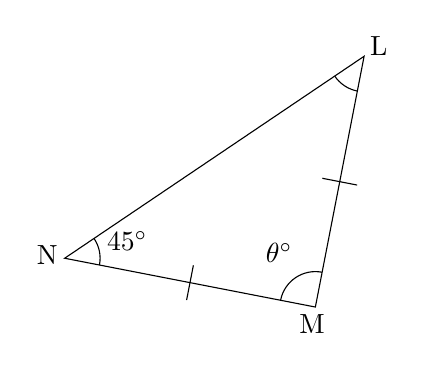
\begin{tikzpicture}[scale=1.5, baseline=(current bounding box.north)]
      \pgfmathsetmacro{\angleA}{45}
      \pgfmathsetmacro{\angleB}{45}
      \pgfmathsetmacro{\angleC}{90}
      \pgfmathsetmacro{\sideC}{3.057816502232179}
      \pgfmathsetmacro{\rotationAngle}{214}
  
    
      \begin{scope}[rotate=\rotationAngle]
        \coordinate (A) at (0,0);
        \coordinate (B) at (\sideC,0);
        \coordinate (C) at (intersection cs: first line={(A)--($(A)+(\angleA:4cm)$)}, second line={(B)--($(B)+(180-\angleB:4cm)$)});
        \draw (A) -- (B) -- (C) -- cycle;
        
        % Mark angles with arcs
        \draw ($(A)!0.3cm!(B)$) arc [start angle=0, end angle=\angleA, radius=0.3cm];
        \draw ($(B)!0.3cm!(C)$) arc [start angle=180-\angleB, end angle=180, radius=0.3cm];
        \draw ($(C)!0.3cm!(A)$) arc [start angle=180+\angleA, end angle=360-\angleB, radius=0.3cm];
        
        % Label angles
        \node at ($(A)!-0.15cm!(B)$) {L};
        \node at ($(B)!-0.15cm!(C)$) {N};
        \node at ($(C)!-0.15cm!(A)$) {M};
        
        % Mark angles in degrees
        \coordinate (midBC) at ($(B)!0.5!(C)$);
        \node at ($(A)!0.55cm!(midBC)$) {};
    
        \coordinate (midAC) at ($(A)!0.5!(C)$);
        \node at ($(B)!0.55cm!(midAC)$) {45$^\circ$};
    
        \coordinate (midAB) at ($(A)!0.5!(B)$);
        \node at ($(C)!0.55cm!(midAB)$) {$\theta ^\circ$};

        % Draw hash mark perpendicular to line AB at its midpoint
        \draw[black] ($(midAC)!1.5mm!90:(A)$)--($(midAC)!1.5mm!-90:(A)$);
              
        % Add hash marks on side AC
        \draw[black] ($(midBC)!1.5mm!90:(B)$)--($(midBC)!1.5mm!-90:(B)$);
              
      \end{scope}
    \end{tikzpicture}
\end{minipage}%
\hfill
\begin{minipage}{0.4\textwidth}
    \begin{align*}
      \angle \text{M} &= 180^\circ - (\angle \text{L} + \angle \text{N}) \\
      &= 180^\circ - (\dotuline{~~~~~~~}^\circ + \dotuline{~~~~~~~}^\circ) \\
      &= 180^\circ - \dotuline{~~~~~~~}^\circ \\
      &= \dotuline{~~~~~~~}^\circ
    \end{align*}
\end{minipage}

\vspace{1cm}\begin{minipage}{0.55\textwidth}
  \refstepcounter{minipagecount}
  \noindent{(\theminipagecount)}\quad
  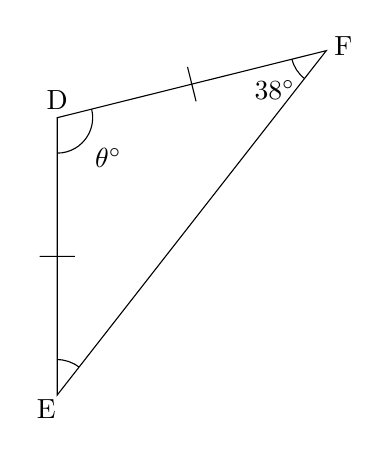
\begin{tikzpicture}[scale=1.5, baseline=(current bounding box.north)]
      \pgfmathsetmacro{\angleA}{38}
      \pgfmathsetmacro{\angleB}{38}
      \pgfmathsetmacro{\angleC}{104}
      \pgfmathsetmacro{\sideC}{3.700062308128377}
      \pgfmathsetmacro{\rotationAngle}{52}
  
    
      \begin{scope}[rotate=\rotationAngle]
        \coordinate (A) at (0,0);
        \coordinate (B) at (\sideC,0);
        \coordinate (C) at (intersection cs: first line={(A)--($(A)+(\angleA:4cm)$)}, second line={(B)--($(B)+(180-\angleB:4cm)$)});
        \draw (A) -- (B) -- (C) -- cycle;
        
        % Mark angles with arcs
        \draw ($(A)!0.3cm!(B)$) arc [start angle=0, end angle=\angleA, radius=0.3cm];
        \draw ($(B)!0.3cm!(C)$) arc [start angle=180-\angleB, end angle=180, radius=0.3cm];
        \draw ($(C)!0.3cm!(A)$) arc [start angle=180+\angleA, end angle=360-\angleB, radius=0.3cm];
        
        % Label angles
        \node at ($(A)!-0.15cm!(B)$) {E};
        \node at ($(B)!-0.15cm!(C)$) {F};
        \node at ($(C)!-0.15cm!(A)$) {D};
        
        % Mark angles in degrees
        \coordinate (midBC) at ($(B)!0.5!(C)$);
        \node at ($(A)!0.55cm!(midBC)$) {};
    
        \coordinate (midAC) at ($(A)!0.5!(C)$);
        \node at ($(B)!0.55cm!(midAC)$) {38$^\circ$};
    
        \coordinate (midAB) at ($(A)!0.5!(B)$);
        \node at ($(C)!0.55cm!(midAB)$) {$\theta ^\circ$};

        % Draw hash mark perpendicular to line AB at its midpoint
        \draw[black] ($(midAC)!1.5mm!90:(A)$)--($(midAC)!1.5mm!-90:(A)$);
              
        % Add hash marks on side AC
        \draw[black] ($(midBC)!1.5mm!90:(B)$)--($(midBC)!1.5mm!-90:(B)$);
              
      \end{scope}
    \end{tikzpicture}
\end{minipage}%
\hfill
\begin{minipage}{0.4\textwidth}
    \begin{align*}
      \angle \text{D} &= 180^\circ - (\angle \text{E} + \angle \text{F}) \\
      &= 180^\circ - (\dotuline{~~~~~~~}^\circ + \dotuline{~~~~~~~}^\circ) \\
      &= 180^\circ - \dotuline{~~~~~~~}^\circ \\
      &= \dotuline{~~~~~~~}^\circ
    \end{align*}
\end{minipage}

\vspace{1cm}\begin{minipage}{0.55\textwidth}
  \refstepcounter{minipagecount}
  \noindent{(\theminipagecount)}\quad
  \begin{tikzpicture}[scale=1.5, baseline=(current bounding box.north)]
      \pgfmathsetmacro{\angleA}{50}
      \pgfmathsetmacro{\angleB}{50}
      \pgfmathsetmacro{\angleC}{80}
      \pgfmathsetmacro{\sideC}{3.4701549360960096}
      \pgfmathsetmacro{\rotationAngle}{152}
  
    
      \begin{scope}[rotate=\rotationAngle]
        \coordinate (A) at (0,0);
        \coordinate (B) at (\sideC,0);
        \coordinate (C) at (intersection cs: first line={(A)--($(A)+(\angleA:4cm)$)}, second line={(B)--($(B)+(180-\angleB:4cm)$)});
        \draw (A) -- (B) -- (C) -- cycle;
        
        % Mark angles with arcs
        \draw ($(A)!0.3cm!(B)$) arc [start angle=0, end angle=\angleA, radius=0.3cm];
        \draw ($(B)!0.3cm!(C)$) arc [start angle=180-\angleB, end angle=180, radius=0.3cm];
        \draw ($(C)!0.3cm!(A)$) arc [start angle=180+\angleA, end angle=360-\angleB, radius=0.3cm];
        
        % Label angles
        \node at ($(A)!-0.15cm!(B)$) {A};
        \node at ($(B)!-0.15cm!(C)$) {C};
        \node at ($(C)!-0.15cm!(A)$) {B};
        
        % Mark angles in degrees
        \coordinate (midBC) at ($(B)!0.5!(C)$);
        \node at ($(A)!0.55cm!(midBC)$) {};
    
        \coordinate (midAC) at ($(A)!0.5!(C)$);
        \node at ($(B)!0.55cm!(midAC)$) {50$^\circ$};
    
        \coordinate (midAB) at ($(A)!0.5!(B)$);
        \node at ($(C)!0.55cm!(midAB)$) {$\theta ^\circ$};

        % Draw hash mark perpendicular to line AB at its midpoint
        \draw[black] ($(midAC)!1.5mm!90:(A)$)--($(midAC)!1.5mm!-90:(A)$);
              
        % Add hash marks on side AC
        \draw[black] ($(midBC)!1.5mm!90:(B)$)--($(midBC)!1.5mm!-90:(B)$);
              
      \end{scope}
    \end{tikzpicture}
\end{minipage}%
\hfill
\begin{minipage}{0.4\textwidth}
    \begin{align*}
      \angle \text{B} &= 180^\circ - (\angle \text{A} + \angle \text{C}) \\
      &= 180^\circ - (\dotuline{~~~~~~~}^\circ + \dotuline{~~~~~~~}^\circ) \\
      &= 180^\circ - \dotuline{~~~~~~~}^\circ \\
      &= \dotuline{~~~~~~~}^\circ
    \end{align*}
\end{minipage}

\vspace{1cm}\begin{minipage}{0.55\textwidth}
  \refstepcounter{minipagecount}
  \noindent{(\theminipagecount)}\quad
  \begin{tikzpicture}[scale=1.5, baseline=(current bounding box.north)]
      \pgfmathsetmacro{\angleA}{56}
      \pgfmathsetmacro{\angleB}{56}
      \pgfmathsetmacro{\angleC}{68}
      \pgfmathsetmacro{\sideC}{3.2837919601011936}
      \pgfmathsetmacro{\rotationAngle}{280}
  
    
      \begin{scope}[rotate=\rotationAngle]
        \coordinate (A) at (0,0);
        \coordinate (B) at (\sideC,0);
        \coordinate (C) at (intersection cs: first line={(A)--($(A)+(\angleA:4cm)$)}, second line={(B)--($(B)+(180-\angleB:4cm)$)});
        \draw (A) -- (B) -- (C) -- cycle;
        
        % Mark angles with arcs
        \draw ($(A)!0.3cm!(B)$) arc [start angle=0, end angle=\angleA, radius=0.3cm];
        \draw ($(B)!0.3cm!(C)$) arc [start angle=180-\angleB, end angle=180, radius=0.3cm];
        \draw ($(C)!0.3cm!(A)$) arc [start angle=180+\angleA, end angle=360-\angleB, radius=0.3cm];
        
        % Label angles
        \node at ($(A)!-0.15cm!(B)$) {E};
        \node at ($(B)!-0.15cm!(C)$) {D};
        \node at ($(C)!-0.15cm!(A)$) {F};
        
        % Mark angles in degrees
        \coordinate (midBC) at ($(B)!0.5!(C)$);
        \node at ($(A)!0.55cm!(midBC)$) {};
    
        \coordinate (midAC) at ($(A)!0.5!(C)$);
        \node at ($(B)!0.55cm!(midAC)$) {56$^\circ$};
    
        \coordinate (midAB) at ($(A)!0.5!(B)$);
        \node at ($(C)!0.55cm!(midAB)$) {$\theta ^\circ$};

        % Draw hash mark perpendicular to line AB at its midpoint
        \draw[black] ($(midAC)!1.5mm!90:(A)$)--($(midAC)!1.5mm!-90:(A)$);
              
        % Add hash marks on side AC
        \draw[black] ($(midBC)!1.5mm!90:(B)$)--($(midBC)!1.5mm!-90:(B)$);
              
      \end{scope}
    \end{tikzpicture}
\end{minipage}%
\hfill
\begin{minipage}{0.4\textwidth}
    \begin{align*}
      \angle \text{F} &= 180^\circ - (\angle \text{E} + \angle \text{D}) \\
      &= 180^\circ - (\dotuline{~~~~~~~}^\circ + \dotuline{~~~~~~~}^\circ) \\
      &= 180^\circ - \dotuline{~~~~~~~}^\circ \\
      &= \dotuline{~~~~~~~}^\circ
    \end{align*}
\end{minipage}

\vspace{1cm}\begin{minipage}{0.55\textwidth}
  \refstepcounter{minipagecount}
  \noindent{(\theminipagecount)}\quad
  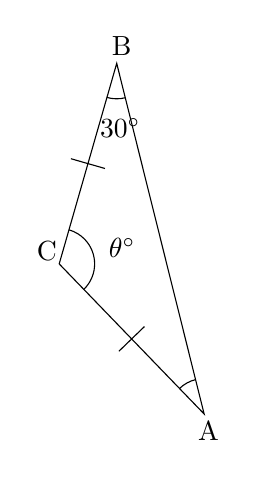
\begin{tikzpicture}[scale=1.5, baseline=(current bounding box.north)]
      \pgfmathsetmacro{\angleA}{30}
      \pgfmathsetmacro{\angleB}{30}
      \pgfmathsetmacro{\angleC}{120}
      \pgfmathsetmacro{\sideC}{3.058848622511449}
      \pgfmathsetmacro{\rotationAngle}{104}
  
    
      \begin{scope}[rotate=\rotationAngle]
        \coordinate (A) at (0,0);
        \coordinate (B) at (\sideC,0);
        \coordinate (C) at (intersection cs: first line={(A)--($(A)+(\angleA:4cm)$)}, second line={(B)--($(B)+(180-\angleB:4cm)$)});
        \draw (A) -- (B) -- (C) -- cycle;
        
        % Mark angles with arcs
        \draw ($(A)!0.3cm!(B)$) arc [start angle=0, end angle=\angleA, radius=0.3cm];
        \draw ($(B)!0.3cm!(C)$) arc [start angle=180-\angleB, end angle=180, radius=0.3cm];
        \draw ($(C)!0.3cm!(A)$) arc [start angle=180+\angleA, end angle=360-\angleB, radius=0.3cm];
        
        % Label angles
        \node at ($(A)!-0.15cm!(B)$) {A};
        \node at ($(B)!-0.15cm!(C)$) {B};
        \node at ($(C)!-0.15cm!(A)$) {C};
        
        % Mark angles in degrees
        \coordinate (midBC) at ($(B)!0.5!(C)$);
        \node at ($(A)!0.55cm!(midBC)$) {};
    
        \coordinate (midAC) at ($(A)!0.5!(C)$);
        \node at ($(B)!0.55cm!(midAC)$) {30$^\circ$};
    
        \coordinate (midAB) at ($(A)!0.5!(B)$);
        \node at ($(C)!0.55cm!(midAB)$) {$\theta ^\circ$};

        % Draw hash mark perpendicular to line AB at its midpoint
        \draw[black] ($(midAC)!1.5mm!90:(A)$)--($(midAC)!1.5mm!-90:(A)$);
              
        % Add hash marks on side AC
        \draw[black] ($(midBC)!1.5mm!90:(B)$)--($(midBC)!1.5mm!-90:(B)$);
              
      \end{scope}
    \end{tikzpicture}
\end{minipage}%
\hfill
\begin{minipage}{0.4\textwidth}
    \begin{align*}
      \angle \text{C} &= 180^\circ - (\angle \text{A} + \angle \text{B}) \\
      &= 180^\circ - (\dotuline{~~~~~~~}^\circ + \dotuline{~~~~~~~}^\circ) \\
      &= 180^\circ - \dotuline{~~~~~~~}^\circ \\
      &= \dotuline{~~~~~~~}^\circ
    \end{align*}
\end{minipage}

\vspace{1cm}\begin{minipage}{0.55\textwidth}
  \refstepcounter{minipagecount}
  \noindent{(\theminipagecount)}\quad
  \begin{tikzpicture}[scale=1.5, baseline=(current bounding box.north)]
      \pgfmathsetmacro{\angleA}{65}
      \pgfmathsetmacro{\angleB}{65}
      \pgfmathsetmacro{\angleC}{50}
      \pgfmathsetmacro{\sideC}{3.2872651552615686}
      \pgfmathsetmacro{\rotationAngle}{356}
  
    
      \begin{scope}[rotate=\rotationAngle]
        \coordinate (A) at (0,0);
        \coordinate (B) at (\sideC,0);
        \coordinate (C) at (intersection cs: first line={(A)--($(A)+(\angleA:4cm)$)}, second line={(B)--($(B)+(180-\angleB:4cm)$)});
        \draw (A) -- (B) -- (C) -- cycle;
        
        % Mark angles with arcs
        \draw ($(A)!0.3cm!(B)$) arc [start angle=0, end angle=\angleA, radius=0.3cm];
        \draw ($(B)!0.3cm!(C)$) arc [start angle=180-\angleB, end angle=180, radius=0.3cm];
        \draw ($(C)!0.3cm!(A)$) arc [start angle=180+\angleA, end angle=360-\angleB, radius=0.3cm];
        
        % Label angles
        \node at ($(A)!-0.15cm!(B)$) {D};
        \node at ($(B)!-0.15cm!(C)$) {F};
        \node at ($(C)!-0.15cm!(A)$) {E};
        
        % Mark angles in degrees
        \coordinate (midBC) at ($(B)!0.5!(C)$);
        \node at ($(A)!0.55cm!(midBC)$) {};
    
        \coordinate (midAC) at ($(A)!0.5!(C)$);
        \node at ($(B)!0.55cm!(midAC)$) {65$^\circ$};
    
        \coordinate (midAB) at ($(A)!0.5!(B)$);
        \node at ($(C)!0.55cm!(midAB)$) {$\theta ^\circ$};

        % Draw hash mark perpendicular to line AB at its midpoint
        \draw[black] ($(midAC)!1.5mm!90:(A)$)--($(midAC)!1.5mm!-90:(A)$);
              
        % Add hash marks on side AC
        \draw[black] ($(midBC)!1.5mm!90:(B)$)--($(midBC)!1.5mm!-90:(B)$);
              
      \end{scope}
    \end{tikzpicture}
\end{minipage}%
\hfill
\begin{minipage}{0.4\textwidth}
    \begin{align*}
      \angle \text{E} &= 180^\circ - (\angle \text{D} + \angle \text{F}) \\
      &= 180^\circ - (\dotuline{~~~~~~~}^\circ + \dotuline{~~~~~~~}^\circ) \\
      &= 180^\circ - \dotuline{~~~~~~~}^\circ \\
      &= \dotuline{~~~~~~~}^\circ
    \end{align*}
\end{minipage}

\vspace{1cm}\begin{minipage}{0.55\textwidth}
  \refstepcounter{minipagecount}
  \noindent{(\theminipagecount)}\quad
  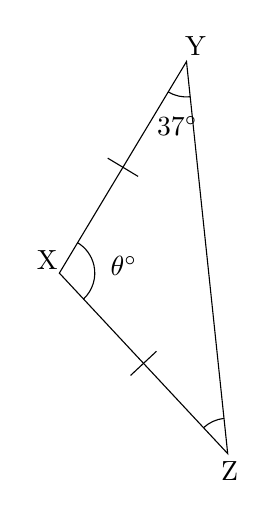
\begin{tikzpicture}[scale=1.5, baseline=(current bounding box.north)]
      \pgfmathsetmacro{\angleA}{37}
      \pgfmathsetmacro{\angleB}{37}
      \pgfmathsetmacro{\angleC}{106}
      \pgfmathsetmacro{\sideC}{3.3376721190936234}
      \pgfmathsetmacro{\rotationAngle}{96}
  
    
      \begin{scope}[rotate=\rotationAngle]
        \coordinate (A) at (0,0);
        \coordinate (B) at (\sideC,0);
        \coordinate (C) at (intersection cs: first line={(A)--($(A)+(\angleA:4cm)$)}, second line={(B)--($(B)+(180-\angleB:4cm)$)});
        \draw (A) -- (B) -- (C) -- cycle;
        
        % Mark angles with arcs
        \draw ($(A)!0.3cm!(B)$) arc [start angle=0, end angle=\angleA, radius=0.3cm];
        \draw ($(B)!0.3cm!(C)$) arc [start angle=180-\angleB, end angle=180, radius=0.3cm];
        \draw ($(C)!0.3cm!(A)$) arc [start angle=180+\angleA, end angle=360-\angleB, radius=0.3cm];
        
        % Label angles
        \node at ($(A)!-0.15cm!(B)$) {Z};
        \node at ($(B)!-0.15cm!(C)$) {Y};
        \node at ($(C)!-0.15cm!(A)$) {X};
        
        % Mark angles in degrees
        \coordinate (midBC) at ($(B)!0.5!(C)$);
        \node at ($(A)!0.55cm!(midBC)$) {};
    
        \coordinate (midAC) at ($(A)!0.5!(C)$);
        \node at ($(B)!0.55cm!(midAC)$) {37$^\circ$};
    
        \coordinate (midAB) at ($(A)!0.5!(B)$);
        \node at ($(C)!0.55cm!(midAB)$) {$\theta ^\circ$};

        % Draw hash mark perpendicular to line AB at its midpoint
        \draw[black] ($(midAC)!1.5mm!90:(A)$)--($(midAC)!1.5mm!-90:(A)$);
              
        % Add hash marks on side AC
        \draw[black] ($(midBC)!1.5mm!90:(B)$)--($(midBC)!1.5mm!-90:(B)$);
              
      \end{scope}
    \end{tikzpicture}
\end{minipage}%
\hfill
\begin{minipage}{0.4\textwidth}
    \begin{align*}
      \angle \text{X} &= 180^\circ - (\angle \text{Z} + \angle \text{Y}) \\
      &= 180^\circ - (\dotuline{~~~~~~~}^\circ + \dotuline{~~~~~~~}^\circ) \\
      &= 180^\circ - \dotuline{~~~~~~~}^\circ \\
      &= \dotuline{~~~~~~~}^\circ
    \end{align*}
\end{minipage}

\vspace{1cm}\begin{minipage}{0.55\textwidth}
  \refstepcounter{minipagecount}
  \noindent{(\theminipagecount)}\quad
  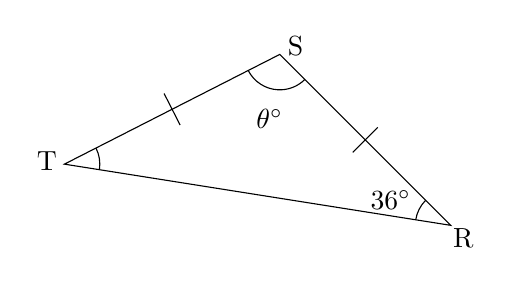
\begin{tikzpicture}[scale=1.5, baseline=(current bounding box.north)]
      \pgfmathsetmacro{\angleA}{36}
      \pgfmathsetmacro{\angleB}{36}
      \pgfmathsetmacro{\angleC}{108}
      \pgfmathsetmacro{\sideC}{3.311272278176497}
      \pgfmathsetmacro{\rotationAngle}{351}
  
    
      \begin{scope}[rotate=\rotationAngle]
        \coordinate (A) at (0,0);
        \coordinate (B) at (\sideC,0);
        \coordinate (C) at (intersection cs: first line={(A)--($(A)+(\angleA:4cm)$)}, second line={(B)--($(B)+(180-\angleB:4cm)$)});
        \draw (A) -- (B) -- (C) -- cycle;
        
        % Mark angles with arcs
        \draw ($(A)!0.3cm!(B)$) arc [start angle=0, end angle=\angleA, radius=0.3cm];
        \draw ($(B)!0.3cm!(C)$) arc [start angle=180-\angleB, end angle=180, radius=0.3cm];
        \draw ($(C)!0.3cm!(A)$) arc [start angle=180+\angleA, end angle=360-\angleB, radius=0.3cm];
        
        % Label angles
        \node at ($(A)!-0.15cm!(B)$) {T};
        \node at ($(B)!-0.15cm!(C)$) {R};
        \node at ($(C)!-0.15cm!(A)$) {S};
        
        % Mark angles in degrees
        \coordinate (midBC) at ($(B)!0.5!(C)$);
        \node at ($(A)!0.55cm!(midBC)$) {};
    
        \coordinate (midAC) at ($(A)!0.5!(C)$);
        \node at ($(B)!0.55cm!(midAC)$) {36$^\circ$};
    
        \coordinate (midAB) at ($(A)!0.5!(B)$);
        \node at ($(C)!0.55cm!(midAB)$) {$\theta ^\circ$};

        % Draw hash mark perpendicular to line AB at its midpoint
        \draw[black] ($(midAC)!1.5mm!90:(A)$)--($(midAC)!1.5mm!-90:(A)$);
              
        % Add hash marks on side AC
        \draw[black] ($(midBC)!1.5mm!90:(B)$)--($(midBC)!1.5mm!-90:(B)$);
              
      \end{scope}
    \end{tikzpicture}
\end{minipage}%
\hfill
\begin{minipage}{0.4\textwidth}
    \begin{align*}
      \angle \text{S} &= 180^\circ - (\angle \text{T} + \angle \text{R}) \\
      &= 180^\circ - (\dotuline{~~~~~~~}^\circ + \dotuline{~~~~~~~}^\circ) \\
      &= 180^\circ - \dotuline{~~~~~~~}^\circ \\
      &= \dotuline{~~~~~~~}^\circ
    \end{align*}
\end{minipage}

\vspace{1cm}\begin{minipage}{0.55\textwidth}
  \refstepcounter{minipagecount}
  \noindent{(\theminipagecount)}\quad
  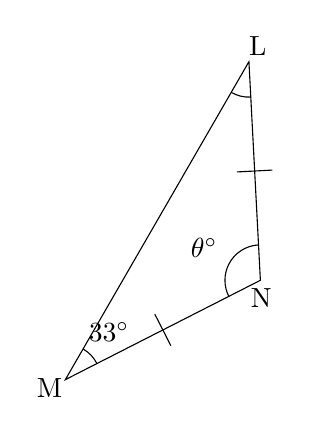
\begin{tikzpicture}[scale=1.5, baseline=(current bounding box.north)]
      \pgfmathsetmacro{\angleA}{33}
      \pgfmathsetmacro{\angleB}{33}
      \pgfmathsetmacro{\angleC}{114}
      \pgfmathsetmacro{\sideC}{3.10789008215247}
      \pgfmathsetmacro{\rotationAngle}{240}
  
    
      \begin{scope}[rotate=\rotationAngle]
        \coordinate (A) at (0,0);
        \coordinate (B) at (\sideC,0);
        \coordinate (C) at (intersection cs: first line={(A)--($(A)+(\angleA:4cm)$)}, second line={(B)--($(B)+(180-\angleB:4cm)$)});
        \draw (A) -- (B) -- (C) -- cycle;
        
        % Mark angles with arcs
        \draw ($(A)!0.3cm!(B)$) arc [start angle=0, end angle=\angleA, radius=0.3cm];
        \draw ($(B)!0.3cm!(C)$) arc [start angle=180-\angleB, end angle=180, radius=0.3cm];
        \draw ($(C)!0.3cm!(A)$) arc [start angle=180+\angleA, end angle=360-\angleB, radius=0.3cm];
        
        % Label angles
        \node at ($(A)!-0.15cm!(B)$) {L};
        \node at ($(B)!-0.15cm!(C)$) {M};
        \node at ($(C)!-0.15cm!(A)$) {N};
        
        % Mark angles in degrees
        \coordinate (midBC) at ($(B)!0.5!(C)$);
        \node at ($(A)!0.55cm!(midBC)$) {};
    
        \coordinate (midAC) at ($(A)!0.5!(C)$);
        \node at ($(B)!0.55cm!(midAC)$) {33$^\circ$};
    
        \coordinate (midAB) at ($(A)!0.5!(B)$);
        \node at ($(C)!0.55cm!(midAB)$) {$\theta ^\circ$};

        % Draw hash mark perpendicular to line AB at its midpoint
        \draw[black] ($(midAC)!1.5mm!90:(A)$)--($(midAC)!1.5mm!-90:(A)$);
              
        % Add hash marks on side AC
        \draw[black] ($(midBC)!1.5mm!90:(B)$)--($(midBC)!1.5mm!-90:(B)$);
              
      \end{scope}
    \end{tikzpicture}
\end{minipage}%
\hfill
\begin{minipage}{0.4\textwidth}
    \begin{align*}
      \angle \text{N} &= 180^\circ - (\angle \text{L} + \angle \text{M}) \\
      &= 180^\circ - (\dotuline{~~~~~~~}^\circ + \dotuline{~~~~~~~}^\circ) \\
      &= 180^\circ - \dotuline{~~~~~~~}^\circ \\
      &= \dotuline{~~~~~~~}^\circ
    \end{align*}
\end{minipage}

\vspace{1cm}\begin{minipage}{0.55\textwidth}
  \refstepcounter{minipagecount}
  \noindent{(\theminipagecount)}\quad
  \begin{tikzpicture}[scale=1.5, baseline=(current bounding box.north)]
      \pgfmathsetmacro{\angleA}{56}
      \pgfmathsetmacro{\angleB}{56}
      \pgfmathsetmacro{\angleC}{68}
      \pgfmathsetmacro{\sideC}{3.3390180617209215}
      \pgfmathsetmacro{\rotationAngle}{211}
  
    
      \begin{scope}[rotate=\rotationAngle]
        \coordinate (A) at (0,0);
        \coordinate (B) at (\sideC,0);
        \coordinate (C) at (intersection cs: first line={(A)--($(A)+(\angleA:4cm)$)}, second line={(B)--($(B)+(180-\angleB:4cm)$)});
        \draw (A) -- (B) -- (C) -- cycle;
        
        % Mark angles with arcs
        \draw ($(A)!0.3cm!(B)$) arc [start angle=0, end angle=\angleA, radius=0.3cm];
        \draw ($(B)!0.3cm!(C)$) arc [start angle=180-\angleB, end angle=180, radius=0.3cm];
        \draw ($(C)!0.3cm!(A)$) arc [start angle=180+\angleA, end angle=360-\angleB, radius=0.3cm];
        
        % Label angles
        \node at ($(A)!-0.15cm!(B)$) {E};
        \node at ($(B)!-0.15cm!(C)$) {F};
        \node at ($(C)!-0.15cm!(A)$) {D};
        
        % Mark angles in degrees
        \coordinate (midBC) at ($(B)!0.5!(C)$);
        \node at ($(A)!0.55cm!(midBC)$) {};
    
        \coordinate (midAC) at ($(A)!0.5!(C)$);
        \node at ($(B)!0.55cm!(midAC)$) {56$^\circ$};
    
        \coordinate (midAB) at ($(A)!0.5!(B)$);
        \node at ($(C)!0.55cm!(midAB)$) {$\theta ^\circ$};

        % Draw hash mark perpendicular to line AB at its midpoint
        \draw[black] ($(midAC)!1.5mm!90:(A)$)--($(midAC)!1.5mm!-90:(A)$);
              
        % Add hash marks on side AC
        \draw[black] ($(midBC)!1.5mm!90:(B)$)--($(midBC)!1.5mm!-90:(B)$);
              
      \end{scope}
    \end{tikzpicture}
\end{minipage}%
\hfill
\begin{minipage}{0.4\textwidth}
    \begin{align*}
      \angle \text{D} &= 180^\circ - (\angle \text{E} + \angle \text{F}) \\
      &= 180^\circ - (\dotuline{~~~~~~~}^\circ + \dotuline{~~~~~~~}^\circ) \\
      &= 180^\circ - \dotuline{~~~~~~~}^\circ \\
      &= \dotuline{~~~~~~~}^\circ
    \end{align*}
\end{minipage}

\vspace{1cm}\begin{minipage}{0.55\textwidth}
  \refstepcounter{minipagecount}
  \noindent{(\theminipagecount)}\quad
  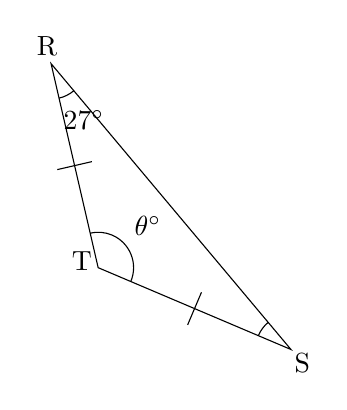
\begin{tikzpicture}[scale=1.5, baseline=(current bounding box.north)]
      \pgfmathsetmacro{\angleA}{27}
      \pgfmathsetmacro{\angleB}{27}
      \pgfmathsetmacro{\angleC}{126}
      \pgfmathsetmacro{\sideC}{3.1595689595331757}
      \pgfmathsetmacro{\rotationAngle}{130}
  
    
      \begin{scope}[rotate=\rotationAngle]
        \coordinate (A) at (0,0);
        \coordinate (B) at (\sideC,0);
        \coordinate (C) at (intersection cs: first line={(A)--($(A)+(\angleA:4cm)$)}, second line={(B)--($(B)+(180-\angleB:4cm)$)});
        \draw (A) -- (B) -- (C) -- cycle;
        
        % Mark angles with arcs
        \draw ($(A)!0.3cm!(B)$) arc [start angle=0, end angle=\angleA, radius=0.3cm];
        \draw ($(B)!0.3cm!(C)$) arc [start angle=180-\angleB, end angle=180, radius=0.3cm];
        \draw ($(C)!0.3cm!(A)$) arc [start angle=180+\angleA, end angle=360-\angleB, radius=0.3cm];
        
        % Label angles
        \node at ($(A)!-0.15cm!(B)$) {S};
        \node at ($(B)!-0.15cm!(C)$) {R};
        \node at ($(C)!-0.15cm!(A)$) {T};
        
        % Mark angles in degrees
        \coordinate (midBC) at ($(B)!0.5!(C)$);
        \node at ($(A)!0.55cm!(midBC)$) {};
    
        \coordinate (midAC) at ($(A)!0.5!(C)$);
        \node at ($(B)!0.55cm!(midAC)$) {27$^\circ$};
    
        \coordinate (midAB) at ($(A)!0.5!(B)$);
        \node at ($(C)!0.55cm!(midAB)$) {$\theta ^\circ$};

        % Draw hash mark perpendicular to line AB at its midpoint
        \draw[black] ($(midAC)!1.5mm!90:(A)$)--($(midAC)!1.5mm!-90:(A)$);
              
        % Add hash marks on side AC
        \draw[black] ($(midBC)!1.5mm!90:(B)$)--($(midBC)!1.5mm!-90:(B)$);
              
      \end{scope}
    \end{tikzpicture}
\end{minipage}%
\hfill
\begin{minipage}{0.4\textwidth}
    \begin{align*}
      \angle \text{T} &= 180^\circ - (\angle \text{S} + \angle \text{R}) \\
      &= 180^\circ - (\dotuline{~~~~~~~}^\circ + \dotuline{~~~~~~~}^\circ) \\
      &= 180^\circ - \dotuline{~~~~~~~}^\circ \\
      &= \dotuline{~~~~~~~}^\circ
    \end{align*}
\end{minipage}

\vspace{1cm}\begin{minipage}{0.55\textwidth}
  \refstepcounter{minipagecount}
  \noindent{(\theminipagecount)}\quad
  \begin{tikzpicture}[scale=1.5, baseline=(current bounding box.north)]
      \pgfmathsetmacro{\angleA}{60}
      \pgfmathsetmacro{\angleB}{60}
      \pgfmathsetmacro{\angleC}{60}
      \pgfmathsetmacro{\sideC}{3.625179955077686}
      \pgfmathsetmacro{\rotationAngle}{56}
  
    
      \begin{scope}[rotate=\rotationAngle]
        \coordinate (A) at (0,0);
        \coordinate (B) at (\sideC,0);
        \coordinate (C) at (intersection cs: first line={(A)--($(A)+(\angleA:4cm)$)}, second line={(B)--($(B)+(180-\angleB:4cm)$)});
        \draw (A) -- (B) -- (C) -- cycle;
        
        % Mark angles with arcs
        \draw ($(A)!0.3cm!(B)$) arc [start angle=0, end angle=\angleA, radius=0.3cm];
        \draw ($(B)!0.3cm!(C)$) arc [start angle=180-\angleB, end angle=180, radius=0.3cm];
        \draw ($(C)!0.3cm!(A)$) arc [start angle=180+\angleA, end angle=360-\angleB, radius=0.3cm];
        
        % Label angles
        \node at ($(A)!-0.15cm!(B)$) {N};
        \node at ($(B)!-0.15cm!(C)$) {M};
        \node at ($(C)!-0.15cm!(A)$) {L};
        
        % Mark angles in degrees
        \coordinate (midBC) at ($(B)!0.5!(C)$);
        \node at ($(A)!0.55cm!(midBC)$) {};
    
        \coordinate (midAC) at ($(A)!0.5!(C)$);
        \node at ($(B)!0.55cm!(midAC)$) {60$^\circ$};
    
        \coordinate (midAB) at ($(A)!0.5!(B)$);
        \node at ($(C)!0.55cm!(midAB)$) {$\theta ^\circ$};

        % Draw hash mark perpendicular to line AB at its midpoint
        \draw[black] ($(midAC)!1.5mm!90:(A)$)--($(midAC)!1.5mm!-90:(A)$);
              
        % Add hash marks on side AC
        \draw[black] ($(midBC)!1.5mm!90:(B)$)--($(midBC)!1.5mm!-90:(B)$);
              
      \end{scope}
    \end{tikzpicture}
\end{minipage}%
\hfill
\begin{minipage}{0.4\textwidth}
    \begin{align*}
      \angle \text{L} &= 180^\circ - (\angle \text{N} + \angle \text{M}) \\
      &= 180^\circ - (\dotuline{~~~~~~~}^\circ + \dotuline{~~~~~~~}^\circ) \\
      &= 180^\circ - \dotuline{~~~~~~~}^\circ \\
      &= \dotuline{~~~~~~~}^\circ
    \end{align*}
\end{minipage}

\vspace{1cm}\begin{minipage}{0.55\textwidth}
  \refstepcounter{minipagecount}
  \noindent{(\theminipagecount)}\quad
  \begin{tikzpicture}[scale=1.5, baseline=(current bounding box.north)]
      \pgfmathsetmacro{\angleA}{54}
      \pgfmathsetmacro{\angleB}{54}
      \pgfmathsetmacro{\angleC}{72}
      \pgfmathsetmacro{\sideC}{3.7768879473046377}
      \pgfmathsetmacro{\rotationAngle}{241}
  
    
      \begin{scope}[rotate=\rotationAngle]
        \coordinate (A) at (0,0);
        \coordinate (B) at (\sideC,0);
        \coordinate (C) at (intersection cs: first line={(A)--($(A)+(\angleA:4cm)$)}, second line={(B)--($(B)+(180-\angleB:4cm)$)});
        \draw (A) -- (B) -- (C) -- cycle;
        
        % Mark angles with arcs
        \draw ($(A)!0.3cm!(B)$) arc [start angle=0, end angle=\angleA, radius=0.3cm];
        \draw ($(B)!0.3cm!(C)$) arc [start angle=180-\angleB, end angle=180, radius=0.3cm];
        \draw ($(C)!0.3cm!(A)$) arc [start angle=180+\angleA, end angle=360-\angleB, radius=0.3cm];
        
        % Label angles
        \node at ($(A)!-0.15cm!(B)$) {E};
        \node at ($(B)!-0.15cm!(C)$) {D};
        \node at ($(C)!-0.15cm!(A)$) {F};
        
        % Mark angles in degrees
        \coordinate (midBC) at ($(B)!0.5!(C)$);
        \node at ($(A)!0.55cm!(midBC)$) {};
    
        \coordinate (midAC) at ($(A)!0.5!(C)$);
        \node at ($(B)!0.55cm!(midAC)$) {54$^\circ$};
    
        \coordinate (midAB) at ($(A)!0.5!(B)$);
        \node at ($(C)!0.55cm!(midAB)$) {$\theta ^\circ$};

        % Draw hash mark perpendicular to line AB at its midpoint
        \draw[black] ($(midAC)!1.5mm!90:(A)$)--($(midAC)!1.5mm!-90:(A)$);
              
        % Add hash marks on side AC
        \draw[black] ($(midBC)!1.5mm!90:(B)$)--($(midBC)!1.5mm!-90:(B)$);
              
      \end{scope}
    \end{tikzpicture}
\end{minipage}%
\hfill
\begin{minipage}{0.4\textwidth}
    \begin{align*}
      \angle \text{F} &= 180^\circ - (\angle \text{E} + \angle \text{D}) \\
      &= 180^\circ - (\dotuline{~~~~~~~}^\circ + \dotuline{~~~~~~~}^\circ) \\
      &= 180^\circ - \dotuline{~~~~~~~}^\circ \\
      &= \dotuline{~~~~~~~}^\circ
    \end{align*}
\end{minipage}

\vspace{1cm}\begin{minipage}{0.55\textwidth}
  \refstepcounter{minipagecount}
  \noindent{(\theminipagecount)}\quad
  \begin{tikzpicture}[scale=1.5, baseline=(current bounding box.north)]
      \pgfmathsetmacro{\angleA}{55}
      \pgfmathsetmacro{\angleB}{55}
      \pgfmathsetmacro{\angleC}{70}
      \pgfmathsetmacro{\sideC}{3.5994699410860087}
      \pgfmathsetmacro{\rotationAngle}{260}
  
    
      \begin{scope}[rotate=\rotationAngle]
        \coordinate (A) at (0,0);
        \coordinate (B) at (\sideC,0);
        \coordinate (C) at (intersection cs: first line={(A)--($(A)+(\angleA:4cm)$)}, second line={(B)--($(B)+(180-\angleB:4cm)$)});
        \draw (A) -- (B) -- (C) -- cycle;
        
        % Mark angles with arcs
        \draw ($(A)!0.3cm!(B)$) arc [start angle=0, end angle=\angleA, radius=0.3cm];
        \draw ($(B)!0.3cm!(C)$) arc [start angle=180-\angleB, end angle=180, radius=0.3cm];
        \draw ($(C)!0.3cm!(A)$) arc [start angle=180+\angleA, end angle=360-\angleB, radius=0.3cm];
        
        % Label angles
        \node at ($(A)!-0.15cm!(B)$) {E};
        \node at ($(B)!-0.15cm!(C)$) {F};
        \node at ($(C)!-0.15cm!(A)$) {D};
        
        % Mark angles in degrees
        \coordinate (midBC) at ($(B)!0.5!(C)$);
        \node at ($(A)!0.55cm!(midBC)$) {};
    
        \coordinate (midAC) at ($(A)!0.5!(C)$);
        \node at ($(B)!0.55cm!(midAC)$) {55$^\circ$};
    
        \coordinate (midAB) at ($(A)!0.5!(B)$);
        \node at ($(C)!0.55cm!(midAB)$) {$\theta ^\circ$};

        % Draw hash mark perpendicular to line AB at its midpoint
        \draw[black] ($(midAC)!1.5mm!90:(A)$)--($(midAC)!1.5mm!-90:(A)$);
              
        % Add hash marks on side AC
        \draw[black] ($(midBC)!1.5mm!90:(B)$)--($(midBC)!1.5mm!-90:(B)$);
              
      \end{scope}
    \end{tikzpicture}
\end{minipage}%
\hfill
\begin{minipage}{0.4\textwidth}
    \begin{align*}
      \angle \text{D} &= 180^\circ - (\angle \text{E} + \angle \text{F}) \\
      &= 180^\circ - (\dotuline{~~~~~~~}^\circ + \dotuline{~~~~~~~}^\circ) \\
      &= 180^\circ - \dotuline{~~~~~~~}^\circ \\
      &= \dotuline{~~~~~~~}^\circ
    \end{align*}
\end{minipage}

\vspace{1cm}\begin{minipage}{0.55\textwidth}
  \refstepcounter{minipagecount}
  \noindent{(\theminipagecount)}\quad
  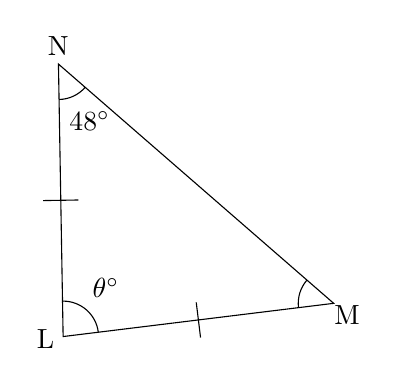
\begin{tikzpicture}[scale=1.5, baseline=(current bounding box.north)]
      \pgfmathsetmacro{\angleA}{48}
      \pgfmathsetmacro{\angleB}{48}
      \pgfmathsetmacro{\angleC}{84}
      \pgfmathsetmacro{\sideC}{3.0873397531936475}
      \pgfmathsetmacro{\rotationAngle}{139}
  
    
      \begin{scope}[rotate=\rotationAngle]
        \coordinate (A) at (0,0);
        \coordinate (B) at (\sideC,0);
        \coordinate (C) at (intersection cs: first line={(A)--($(A)+(\angleA:4cm)$)}, second line={(B)--($(B)+(180-\angleB:4cm)$)});
        \draw (A) -- (B) -- (C) -- cycle;
        
        % Mark angles with arcs
        \draw ($(A)!0.3cm!(B)$) arc [start angle=0, end angle=\angleA, radius=0.3cm];
        \draw ($(B)!0.3cm!(C)$) arc [start angle=180-\angleB, end angle=180, radius=0.3cm];
        \draw ($(C)!0.3cm!(A)$) arc [start angle=180+\angleA, end angle=360-\angleB, radius=0.3cm];
        
        % Label angles
        \node at ($(A)!-0.15cm!(B)$) {M};
        \node at ($(B)!-0.15cm!(C)$) {N};
        \node at ($(C)!-0.15cm!(A)$) {L};
        
        % Mark angles in degrees
        \coordinate (midBC) at ($(B)!0.5!(C)$);
        \node at ($(A)!0.55cm!(midBC)$) {};
    
        \coordinate (midAC) at ($(A)!0.5!(C)$);
        \node at ($(B)!0.55cm!(midAC)$) {48$^\circ$};
    
        \coordinate (midAB) at ($(A)!0.5!(B)$);
        \node at ($(C)!0.55cm!(midAB)$) {$\theta ^\circ$};

        % Draw hash mark perpendicular to line AB at its midpoint
        \draw[black] ($(midAC)!1.5mm!90:(A)$)--($(midAC)!1.5mm!-90:(A)$);
              
        % Add hash marks on side AC
        \draw[black] ($(midBC)!1.5mm!90:(B)$)--($(midBC)!1.5mm!-90:(B)$);
              
      \end{scope}
    \end{tikzpicture}
\end{minipage}%
\hfill
\begin{minipage}{0.4\textwidth}
    \begin{align*}
      \angle \text{L} &= 180^\circ - (\angle \text{M} + \angle \text{N}) \\
      &= 180^\circ - (\dotuline{~~~~~~~}^\circ + \dotuline{~~~~~~~}^\circ) \\
      &= 180^\circ - \dotuline{~~~~~~~}^\circ \\
      &= \dotuline{~~~~~~~}^\circ
    \end{align*}
\end{minipage}

\vspace{1cm}\begin{minipage}{0.55\textwidth}
  \refstepcounter{minipagecount}
  \noindent{(\theminipagecount)}\quad
  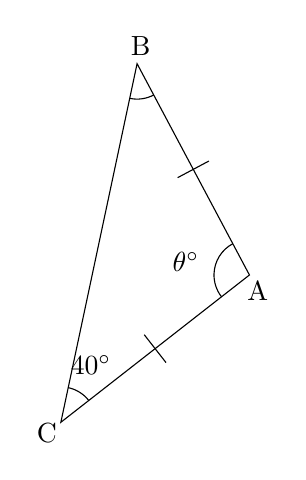
\begin{tikzpicture}[scale=1.5, baseline=(current bounding box.north)]
      \pgfmathsetmacro{\angleA}{40}
      \pgfmathsetmacro{\angleB}{40}
      \pgfmathsetmacro{\angleC}{100}
      \pgfmathsetmacro{\sideC}{3.1036626032027765}
      \pgfmathsetmacro{\rotationAngle}{258}
  
    
      \begin{scope}[rotate=\rotationAngle]
        \coordinate (A) at (0,0);
        \coordinate (B) at (\sideC,0);
        \coordinate (C) at (intersection cs: first line={(A)--($(A)+(\angleA:4cm)$)}, second line={(B)--($(B)+(180-\angleB:4cm)$)});
        \draw (A) -- (B) -- (C) -- cycle;
        
        % Mark angles with arcs
        \draw ($(A)!0.3cm!(B)$) arc [start angle=0, end angle=\angleA, radius=0.3cm];
        \draw ($(B)!0.3cm!(C)$) arc [start angle=180-\angleB, end angle=180, radius=0.3cm];
        \draw ($(C)!0.3cm!(A)$) arc [start angle=180+\angleA, end angle=360-\angleB, radius=0.3cm];
        
        % Label angles
        \node at ($(A)!-0.15cm!(B)$) {B};
        \node at ($(B)!-0.15cm!(C)$) {C};
        \node at ($(C)!-0.15cm!(A)$) {A};
        
        % Mark angles in degrees
        \coordinate (midBC) at ($(B)!0.5!(C)$);
        \node at ($(A)!0.55cm!(midBC)$) {};
    
        \coordinate (midAC) at ($(A)!0.5!(C)$);
        \node at ($(B)!0.55cm!(midAC)$) {40$^\circ$};
    
        \coordinate (midAB) at ($(A)!0.5!(B)$);
        \node at ($(C)!0.55cm!(midAB)$) {$\theta ^\circ$};

        % Draw hash mark perpendicular to line AB at its midpoint
        \draw[black] ($(midAC)!1.5mm!90:(A)$)--($(midAC)!1.5mm!-90:(A)$);
              
        % Add hash marks on side AC
        \draw[black] ($(midBC)!1.5mm!90:(B)$)--($(midBC)!1.5mm!-90:(B)$);
              
      \end{scope}
    \end{tikzpicture}
\end{minipage}%
\hfill
\begin{minipage}{0.4\textwidth}
    \begin{align*}
      \angle \text{A} &= 180^\circ - (\angle \text{B} + \angle \text{C}) \\
      &= 180^\circ - (\dotuline{~~~~~~~}^\circ + \dotuline{~~~~~~~}^\circ) \\
      &= 180^\circ - \dotuline{~~~~~~~}^\circ \\
      &= \dotuline{~~~~~~~}^\circ
    \end{align*}
\end{minipage}

\vspace{1cm}\begin{minipage}{0.55\textwidth}
  \refstepcounter{minipagecount}
  \noindent{(\theminipagecount)}\quad
  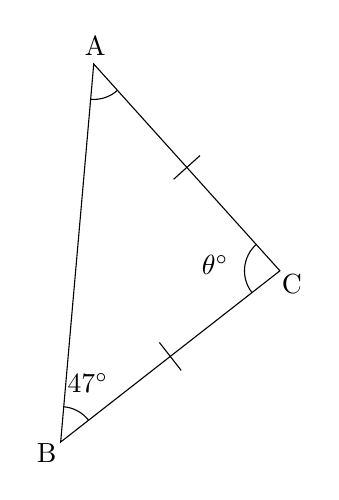
\begin{tikzpicture}[scale=1.5, baseline=(current bounding box.north)]
      \pgfmathsetmacro{\angleA}{47}
      \pgfmathsetmacro{\angleB}{47}
      \pgfmathsetmacro{\angleC}{86}
      \pgfmathsetmacro{\sideC}{3.2126475156581504}
      \pgfmathsetmacro{\rotationAngle}{265}
  
    
      \begin{scope}[rotate=\rotationAngle]
        \coordinate (A) at (0,0);
        \coordinate (B) at (\sideC,0);
        \coordinate (C) at (intersection cs: first line={(A)--($(A)+(\angleA:4cm)$)}, second line={(B)--($(B)+(180-\angleB:4cm)$)});
        \draw (A) -- (B) -- (C) -- cycle;
        
        % Mark angles with arcs
        \draw ($(A)!0.3cm!(B)$) arc [start angle=0, end angle=\angleA, radius=0.3cm];
        \draw ($(B)!0.3cm!(C)$) arc [start angle=180-\angleB, end angle=180, radius=0.3cm];
        \draw ($(C)!0.3cm!(A)$) arc [start angle=180+\angleA, end angle=360-\angleB, radius=0.3cm];
        
        % Label angles
        \node at ($(A)!-0.15cm!(B)$) {A};
        \node at ($(B)!-0.15cm!(C)$) {B};
        \node at ($(C)!-0.15cm!(A)$) {C};
        
        % Mark angles in degrees
        \coordinate (midBC) at ($(B)!0.5!(C)$);
        \node at ($(A)!0.55cm!(midBC)$) {};
    
        \coordinate (midAC) at ($(A)!0.5!(C)$);
        \node at ($(B)!0.55cm!(midAC)$) {47$^\circ$};
    
        \coordinate (midAB) at ($(A)!0.5!(B)$);
        \node at ($(C)!0.55cm!(midAB)$) {$\theta ^\circ$};

        % Draw hash mark perpendicular to line AB at its midpoint
        \draw[black] ($(midAC)!1.5mm!90:(A)$)--($(midAC)!1.5mm!-90:(A)$);
              
        % Add hash marks on side AC
        \draw[black] ($(midBC)!1.5mm!90:(B)$)--($(midBC)!1.5mm!-90:(B)$);
              
      \end{scope}
    \end{tikzpicture}
\end{minipage}%
\hfill
\begin{minipage}{0.4\textwidth}
    \begin{align*}
      \angle \text{C} &= 180^\circ - (\angle \text{A} + \angle \text{B}) \\
      &= 180^\circ - (\dotuline{~~~~~~~}^\circ + \dotuline{~~~~~~~}^\circ) \\
      &= 180^\circ - \dotuline{~~~~~~~}^\circ \\
      &= \dotuline{~~~~~~~}^\circ
    \end{align*}
\end{minipage}

\vspace{1cm}\begin{minipage}{0.55\textwidth}
  \refstepcounter{minipagecount}
  \noindent{(\theminipagecount)}\quad
  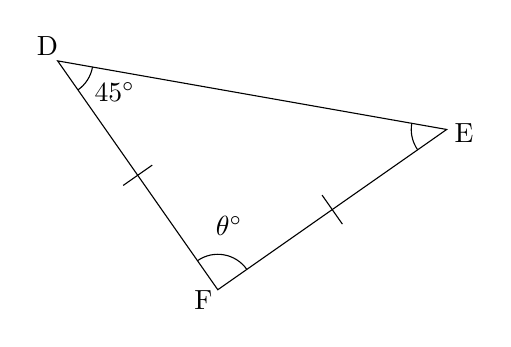
\begin{tikzpicture}[scale=1.5, baseline=(current bounding box.north)]
      \pgfmathsetmacro{\angleA}{45}
      \pgfmathsetmacro{\angleB}{45}
      \pgfmathsetmacro{\angleC}{90}
      \pgfmathsetmacro{\sideC}{3.344419444108279}
      \pgfmathsetmacro{\rotationAngle}{170}
  
    
      \begin{scope}[rotate=\rotationAngle]
        \coordinate (A) at (0,0);
        \coordinate (B) at (\sideC,0);
        \coordinate (C) at (intersection cs: first line={(A)--($(A)+(\angleA:4cm)$)}, second line={(B)--($(B)+(180-\angleB:4cm)$)});
        \draw (A) -- (B) -- (C) -- cycle;
        
        % Mark angles with arcs
        \draw ($(A)!0.3cm!(B)$) arc [start angle=0, end angle=\angleA, radius=0.3cm];
        \draw ($(B)!0.3cm!(C)$) arc [start angle=180-\angleB, end angle=180, radius=0.3cm];
        \draw ($(C)!0.3cm!(A)$) arc [start angle=180+\angleA, end angle=360-\angleB, radius=0.3cm];
        
        % Label angles
        \node at ($(A)!-0.15cm!(B)$) {E};
        \node at ($(B)!-0.15cm!(C)$) {D};
        \node at ($(C)!-0.15cm!(A)$) {F};
        
        % Mark angles in degrees
        \coordinate (midBC) at ($(B)!0.5!(C)$);
        \node at ($(A)!0.55cm!(midBC)$) {};
    
        \coordinate (midAC) at ($(A)!0.5!(C)$);
        \node at ($(B)!0.55cm!(midAC)$) {45$^\circ$};
    
        \coordinate (midAB) at ($(A)!0.5!(B)$);
        \node at ($(C)!0.55cm!(midAB)$) {$\theta ^\circ$};

        % Draw hash mark perpendicular to line AB at its midpoint
        \draw[black] ($(midAC)!1.5mm!90:(A)$)--($(midAC)!1.5mm!-90:(A)$);
              
        % Add hash marks on side AC
        \draw[black] ($(midBC)!1.5mm!90:(B)$)--($(midBC)!1.5mm!-90:(B)$);
              
      \end{scope}
    \end{tikzpicture}
\end{minipage}%
\hfill
\begin{minipage}{0.4\textwidth}
    \begin{align*}
      \angle \text{F} &= 180^\circ - (\angle \text{E} + \angle \text{D}) \\
      &= 180^\circ - (\dotuline{~~~~~~~}^\circ + \dotuline{~~~~~~~}^\circ) \\
      &= 180^\circ - \dotuline{~~~~~~~}^\circ \\
      &= \dotuline{~~~~~~~}^\circ
    \end{align*}
\end{minipage}

\vspace{1cm}\begin{minipage}{0.55\textwidth}
  \refstepcounter{minipagecount}
  \noindent{(\theminipagecount)}\quad
  \begin{tikzpicture}[scale=1.5, baseline=(current bounding box.north)]
      \pgfmathsetmacro{\angleA}{47}
      \pgfmathsetmacro{\angleB}{47}
      \pgfmathsetmacro{\angleC}{86}
      \pgfmathsetmacro{\sideC}{3.7805065964642273}
      \pgfmathsetmacro{\rotationAngle}{301}
  
    
      \begin{scope}[rotate=\rotationAngle]
        \coordinate (A) at (0,0);
        \coordinate (B) at (\sideC,0);
        \coordinate (C) at (intersection cs: first line={(A)--($(A)+(\angleA:4cm)$)}, second line={(B)--($(B)+(180-\angleB:4cm)$)});
        \draw (A) -- (B) -- (C) -- cycle;
        
        % Mark angles with arcs
        \draw ($(A)!0.3cm!(B)$) arc [start angle=0, end angle=\angleA, radius=0.3cm];
        \draw ($(B)!0.3cm!(C)$) arc [start angle=180-\angleB, end angle=180, radius=0.3cm];
        \draw ($(C)!0.3cm!(A)$) arc [start angle=180+\angleA, end angle=360-\angleB, radius=0.3cm];
        
        % Label angles
        \node at ($(A)!-0.15cm!(B)$) {Z};
        \node at ($(B)!-0.15cm!(C)$) {X};
        \node at ($(C)!-0.15cm!(A)$) {Y};
        
        % Mark angles in degrees
        \coordinate (midBC) at ($(B)!0.5!(C)$);
        \node at ($(A)!0.55cm!(midBC)$) {};
    
        \coordinate (midAC) at ($(A)!0.5!(C)$);
        \node at ($(B)!0.55cm!(midAC)$) {47$^\circ$};
    
        \coordinate (midAB) at ($(A)!0.5!(B)$);
        \node at ($(C)!0.55cm!(midAB)$) {$\theta ^\circ$};

        % Draw hash mark perpendicular to line AB at its midpoint
        \draw[black] ($(midAC)!1.5mm!90:(A)$)--($(midAC)!1.5mm!-90:(A)$);
              
        % Add hash marks on side AC
        \draw[black] ($(midBC)!1.5mm!90:(B)$)--($(midBC)!1.5mm!-90:(B)$);
              
      \end{scope}
    \end{tikzpicture}
\end{minipage}%
\hfill
\begin{minipage}{0.4\textwidth}
    \begin{align*}
      \angle \text{Y} &= 180^\circ - (\angle \text{Z} + \angle \text{X}) \\
      &= 180^\circ - (\dotuline{~~~~~~~}^\circ + \dotuline{~~~~~~~}^\circ) \\
      &= 180^\circ - \dotuline{~~~~~~~}^\circ \\
      &= \dotuline{~~~~~~~}^\circ
    \end{align*}
\end{minipage}

\vspace{1cm}

\end{document}
